\documentclass[tikz,border=12pt]{standalone}

\begin{document}

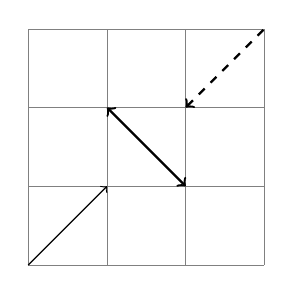
\begin{tikzpicture}
\draw[help lines](0,0) grid (3,3);
\draw[->] (0,0) -- (1,1);
\draw[<->, thick] (2,1) -- (1,2);
\draw[<-, thick, dashed] (2,2) -- (3,3);
\end{tikzpicture}

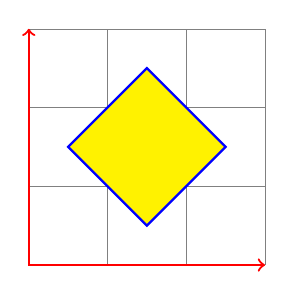
\begin{tikzpicture}
\draw[help lines](0,0) grid (3,3);
% axes:
\draw[<->, thick, red] (0,3) -- (0,0) -- (3,0);
% diamond:
\draw[thick, blue, fill=yellow]
 (1.5,0.5) -- (2.5,1.5) --
 (1.5,2.5) -- (0.5,1.5) --
 cycle; % cierra el camino	
\end{tikzpicture}

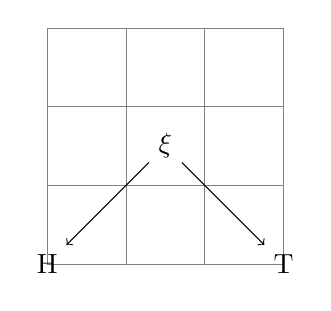
\begin{tikzpicture}
\draw[help lines](0,0) grid (3,3);
\node (h) at (0,0) {H};
\node (x) at (1.5,1.5) {$\xi$};
\node (t) at (3,0) {T};
\draw[->] (x) -- (h);
\draw[->] (x) -- (t);
\end{tikzpicture}

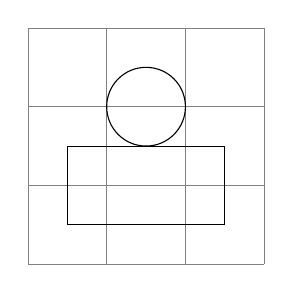
\begin{tikzpicture}
\draw[help lines](0,0) grid (3,3);
\draw (1.5,2.0) circle (0.5); % dibujar un circulo que su centro este en (1.5,2.0) y tenga de radio 0.5
\draw (0.5,0.5) rectangle (2.5,1.5); % dibujar rectángulo cuyo vértice de abajo a la izquierda empieza en (0.5,0.5) y el vértice de arriba a la derecha está en (2.5,1.5)
\end{tikzpicture}

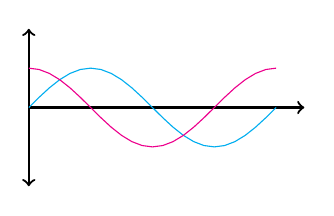
\begin{tikzpicture}[scale=0.5]
% eje y
\draw[<->, thick] (0,2) -- (0,-2);
% eje x
\draw[->, thick] (0,0) -- (7,0);
% curvas
\draw[cyan,domain=0:2*pi]
plot(\x,{sin(\x r)});
\draw[magenta,domain=0:2*pi]
plot(\x,{cos(\x r)});
\end{tikzpicture}

\end{document}